% =============================================================================
%  Avant-propos — le projet, la stratification des théories, le but
% =============================================================================
\section*{Avant-propos --- le projet}
\addcontentsline{toc}{section}{Avant-propos --- le projet}

\paragraph{Objectif} Reformaliser \emph{intégralement} le livre \emph{Théorie
des ensembles} de N.~Bourbaki dans du code, chaque résultat nommé (définition,
axiome, critère, proposition, théorème, corollaire) devenant un objet
\theoreme{} \textbf{certifié par un noyau de preuve LCF} écrit en Python. La
ligne directrice est une exigence d'\emph{adéquation} : « démontré dans le
livre » doit coïncider avec « vérifié par la machine ». Un résultat n'est
déclaré \emph{fait} que s'il est \emph{clos} (zéro hypothèse non déchargée) ---
ou \emph{conditionnel honnête} (voir plus bas) --- et que son énoncé est
exactement celui de Bourbaki ; sinon il reste \emph{partiel}.

% --------------------------------------------------------------------------
\subsection*{L'idée centrale : des théories emboîtées}
\addcontentsline{toc}{subsection}{L'idée centrale : des théories emboîtées}

Bourbaki ne raisonne jamais « dans les mathématiques » en général : il raisonne
\emph{dans une théorie} précise --- un langage muni d'une liste finie d'axiomes.
Et il les construit \textbf{par couches de force croissante}. Une théorie
$\mathcal{T}'$ est dite \emph{plus forte} que $\mathcal{T}$ lorsque tout signe
et tout axiome de $\mathcal{T}$ est un signe, un axiome \emph{ou un théorème} de
$\mathcal{T}'$. On obtient ainsi une tour :
\[
  \underbrace{\text{logique}}_{\text{S1--S7}}\ \subset\
  \text{+ égalité}\ \subset\
  \underbrace{\text{ensembles}}_{\text{extensionnalité, couple, sélection-réunion,\ldots}}\ \subset\
  \text{+ ordre}\ \subset\ \text{+ cardinaux}\ \subset\ \text{structures}.
\]

Ce rapport est \emph{organisé selon cette tour}, et non par ordre
chronologique de travail. La discipline qui en découle est absolue :

\begin{quote}
\itshape on démontre chaque résultat dans la théorie \textbf{la plus faible} qui
le permet.
\end{quote}

Un théorème purement logique se prouve \emph{dans la théorie logique}, avec les
seuls schémas S1--S7 --- il est interdit d'aller chercher un axiome ensembliste
« au-dessus ». La récompense est double : chaque résultat est \emph{localisé}
(on lit exactement de quels axiomes il dépend, et de rien d'autre), et il
\emph{s'hérite vers le haut} (prouvé une fois en bas, il vaut dans toutes les
théories plus fortes, sans jamais être redémontré).

% --------------------------------------------------------------------------
\subsection*{Le noyau LCF et la frontière de confiance}
\addcontentsline{toc}{subsection}{Le noyau LCF et la frontière de confiance}

Le c\oe ur de confiance est minuscule et isolé
(\texttt{bourbaki/logique/i\_2\_criteres\_C/noyau/}). Un \theoreme{} y est un
\emph{séquent} $\Gamma \vdash B$ (sous les hypothèses $\Gamma$, la relation $B$
est démontrable). Il ne peut être créé \emph{que} par les primitives du noyau,
exposées sous le préfixe \Nstar{} --- chacune étant \emph{exactement} une règle
sûre de Bourbaki :

\begin{center}\small
\begin{tabular}{@{}ll@{}}
\toprule
Primitive \Nstar{} & Règle de Bourbaki \\
\midrule
\texttt{assume} & introduction d'hypothèse $\{A\}\vdash A$ \\
\texttt{s1}\,\ldots\,\texttt{s7} & les sept schémas logiques (PDF p.~33--38) \\
\texttt{axiome(T,A)} & $\vdash A$ si $A$ est un axiome explicite de $\mathcal{T}$ \\
\texttt{modus\_ponens} & détachement (critère C1) \\
\texttt{loi\_deduction} & théorème de la déduction (C6) \\
\texttt{generalisation} & passage au $\forall$ (C27) \\
\texttt{existe\_temoin} & le $\tau$ de Hilbert (schéma S5) \\
\texttt{instancie} & substitution (critère CS) \\
\bottomrule
\end{tabular}
\end{center}

La classe \theoreme{} est verrouillée par une clé privée (\texttt{\_CLE}) : il
est \emph{impossible} de fabriquer un théorème à la main, de contourner le
constructeur ou de \emph{monkeypatcher} le noyau. Toute la mathématique du
projet (des milliers de lemmes) vit \emph{au-dessus} de cette frontière : ce
sont des \emph{tactiques} dont le seul pouvoir est d'enchaîner les primitives.
La figure~\ref{fig:couches} schématise ces couches.

\begin{figure}[h]
  \centering
  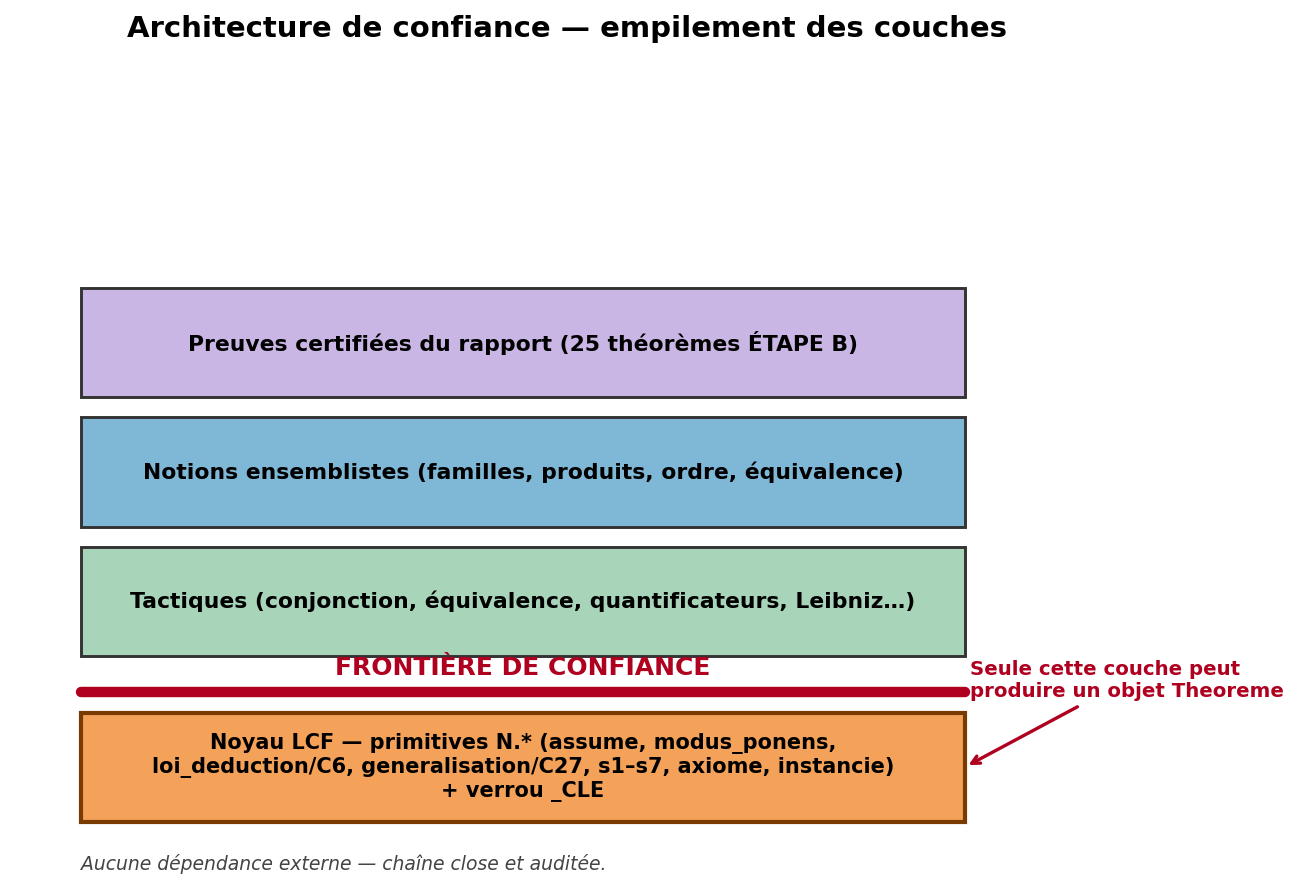
\includegraphics[width=0.82\textwidth]{figures/architecture_noyau}
  \caption{Architecture en couches. Seule la couche \noyau{} (primitives
  \Nstar{}, verrou \texttt{\_CLE}) peut produire un \theoreme{}. Tout le reste
  --- tactiques, notions ensemblistes, preuves de ce rapport --- est au-dessus
  de la frontière de confiance et ne peut que \emph{composer} des appels
  certifiés.}
  \label{fig:couches}
\end{figure}

\paragraph{Où vivent les axiomes} La couche logique (\texttt{s1}--\texttt{s7})
ne prend \emph{aucune} théorie en argument : un résultat qui ne fait aucun appel
à \texttt{axiome(T,$\cdot$)} est, de fait, un théorème de la \emph{logique pure},
valide dans toute théorie. Les axiomes \emph{propres} sont invoqués par
\texttt{axiome}. La théorie ensembliste de référence vaut exactement
\textbf{22~axiomes} (\texttt{theorie\_ensembles().axiomes == 22}) ; elle mêle
trois \emph{vrais} axiomes de Bourbaki (extensionnalité, couple, ensemble des
parties) et dix-neuf axiomes \emph{définitionnels} (qui posent la propriété
caractéristique d'un symbole construit : $\cup$, $\cap$, $\times$, domaine,
image, $\bigcup_\iota$, quotient, \dots). Chaque résultat de ce rapport a été
vérifié sans modifier ce compte~: les caractérisations auxiliaires (membership
de $E^I$, des intervalles, des termes opaques) vivent dans des \emph{théories
locales} séparées, plus fortes, qui n'altèrent pas l'invariant.

\paragraph{Hypothèses honnêtes} Lorsqu'un énoncé du livre est \emph{conditionnel}
(« si $f$ applique $A$ dans $B$, alors \dots »), la formalisation garde ces
antécédents comme \emph{hypothèses explicites} du séquent, ou les décharge en
une implication close. La règle absolue : \textbf{la conclusion n'apparaît
jamais parmi les hypothèses} (sinon ce serait la tautologie $R\vdash R$), et
aucune hypothèse parasite n'est ajoutée (uniquement les antécédents réellement
\emph{consommés} par la preuve de Bourbaki). Un théorème « clos sous hypothèses
honnêtes » est un \emph{fait conditionnel légitime}, fidèle à l'énoncé --- jamais
un résultat tronqué déguisé.

% --------------------------------------------------------------------------
\subsection*{Le but : un substrat pour une IA bâtisseuse de théories}
\addcontentsline{toc}{subsection}{Le but : un substrat pour une IA bâtisseuse de théories}

Certifier le livre n'est pas la fin ; c'est le moyen. L'objectif est de
constituer un \textbf{corpus d'entraînement} pour une intelligence artificielle
capable, à terme, de \emph{construire des théories par elle-même} à partir
d'axiomes. Cela impose une exigence inhabituelle pour une bibliothèque de
preuves : le corpus doit être \emph{riche en information de construction}, pas
seulement « la preuve passe ». On y consigne donc, pour chaque couche :
\emph{comment} la théorie a été bâtie, \emph{les erreurs} commises et leur
correction, et \emph{pourquoi} chaque choix a été fait. Les impasses (capture de
variable, énoncé faux refusé par le noyau, hypothèse inerte, tautologie
déguisée) ne sont pas du bruit à masquer : ce sont des \emph{données de première
classe}. L'annexe « Journal des erreurs \& leçons » les rassemble ; chaque
partie en signale les épisodes marquants au fil de l'eau.

% --------------------------------------------------------------------------
\subsection*{Méthode : fidélité au livre, traçabilité, structure}
\addcontentsline{toc}{subsection}{Méthode : fidélité au livre, traçabilité, structure}

\paragraph{Fidélité} Le noyau garantit la \emph{soundness} (aucun faux
théorème) mais \emph{pas} la \emph{fidélité} (énoncé $=$ Bourbaki) : celle-ci
repose sur une relecture directe du PDF du livre pour \emph{chaque} notion. En
cas de conflit, le \textbf{PDF prime} pour la fidélité, le \textbf{noyau
tranche} pour la soundness ; tout écart est consigné en annexe.

\paragraph{Traçabilité ligne-à-ligne} Chaque notion porte un marqueur
machine-lisible \texttt{@livre} (repère Bourbaki + intervalle de lignes + page
physique du scan). En triant tout le corpus par (chapitre, page, ligne), un
\emph{intervalle non couvert} signale une notion oubliée : \emph{la citation est
le détecteur de trous}.

\paragraph{Structure} L'arborescence du code \emph{calque la table des matières}
(chapitre $\to$ section $\to$ sous-section) ; un trou de couverture devient
visible \emph{structurellement} (dossier vide $=$ résultat pas encore
formalisé). Deux règles d'hygiène : un fichier $=$ une responsabilité,
$\leq 300$ lignes ; et $\leq 10$ entrées par dossier (fichiers et sous-dossiers
confondus). Le répertoire \texttt{tests/} reflète \texttt{bourbaki/} à
l'identique.

\paragraph{Performance et mur algorithmique} Les preuves \emph{cardinales
profondes} (cardinal d'assemblages $\tau$ à $\sim 1.5\times 10^{5}$ n\oe uds)
coûtent plusieurs centaines de secondes, dominées par le hachage de formules
lors de la substitution (figure~\ref{fig:memo}) : un mur \emph{algorithmique}.
La mémoïsation de la substitution pure du noyau apporte un gain mesuré (28~\%)
mais ne le franchit pas ; la stratégie a donc été de \emph{pivoter} vers les
résultats ensemblistes et d'ordre (chacun certifié en moins d'une seconde), en
documentant les cardinaux profonds comme partiels bloqués par la performance.

\begin{figure}[h]
  \centering
  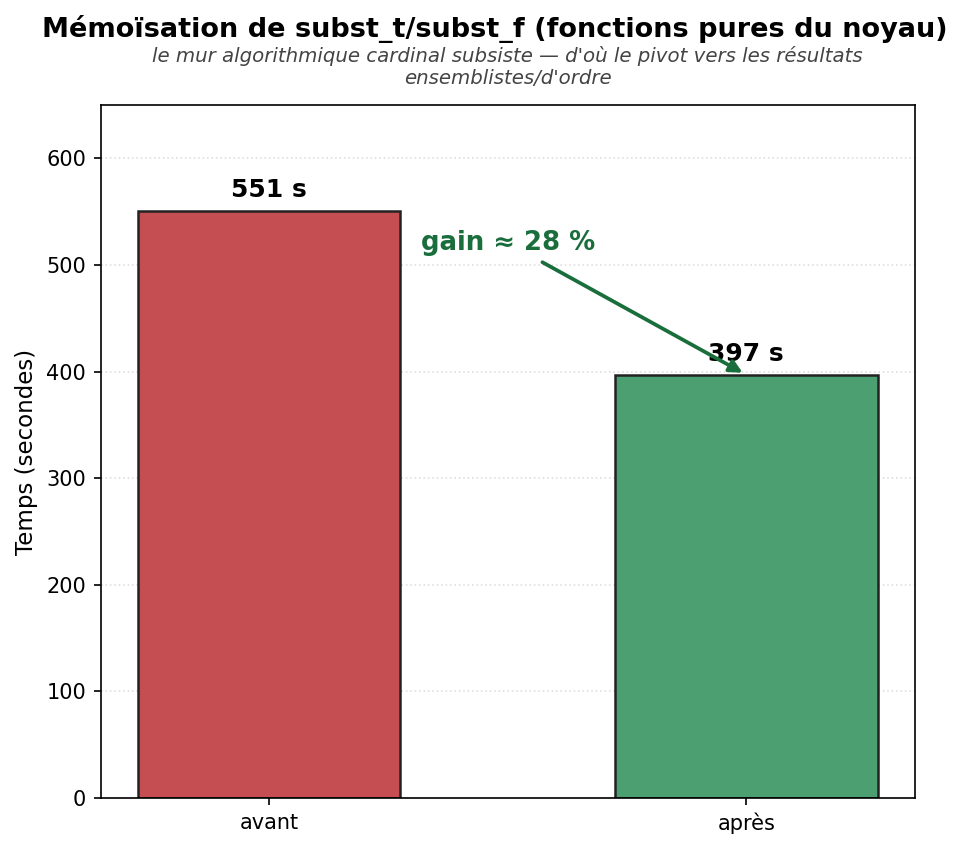
\includegraphics[width=0.72\textwidth]{figures/memoisation_subst}
  \caption{Effet de la mémoïsation de la substitution pure du noyau
  (\texttt{subst\_t}/\texttt{subst\_f}, déterministes, sans effet de bord) sur un
  témoin de preuve cardinale. Gain réel, mur algorithmique persistant : d'où le
  pivot vers les résultats ensemblistes et d'ordre.}
  \label{fig:memo}
\end{figure}

% --------------------------------------------------------------------------
\subsection*{Plan du rapport}
\addcontentsline{toc}{subsection}{Plan du rapport}

Le rapport suit la tour des théories. La \textbf{Partie~I} pose la théorie
logique (langage, $\tau$, quantificateurs définis, schémas S1--S7, détachement).
La \textbf{Partie~II} \emph{augmente} la théorie en y ajoutant les axiomes
ensemblistes et développe l'algèbre des ensembles, les couples et produits, les
correspondances et fonctions, les familles et les relations d'équivalence. La
\textbf{Partie~III} traite l'ordre, le bon ordre et les cardinaux comme
\emph{extensions définitionnelles} (peu ou pas de nouveaux axiomes). La
\textbf{Partie~IV} aborde les structures. Une \textbf{annexe} consolide le
journal des erreurs et des leçons méthodologiques. Pour chaque résultat : énoncé
de Bourbaki, ce qui est formalisé, la stratégie de preuve par les primitives
\Nstar{}, et le statut (clos / clos sous hypothèses honnêtes).
